\section{Teilversuch 5: Strahlung eines Hohlraumstrahers}
	Raumtemperatur $T_0 = \SI{29.0(1)}{\celsius}$

	Fehler bei Messung der Spannung $\Delta V = \SI{2}{\micro\volt}$\\
	Fehler bei der Temperatur $\Delta \theta = \SI{0.1}{\celsius} = \SI{0.1}{\kelvin}$
	\begin{equation*}
		\begin{tabu}{l *{11}{c}}
			\toprule
			\theta/\si{\celsius} & 80 & 100 & 130 & 160 & 190 & 210 & 240 & 270 & 300 & 330 & 350 \\
			\midrule
			V/\si{\micro\volt} & 10 & 18 & 25 & 52 & 63 & 79 & 108 & 139 & 174 & 222 & 250 \\
			\bottomrule
		\end{tabu}
	\end{equation*}
	Fehler für $x = (T^4 - T_0^4)$ ist gegeben durch:
	\begin{align}
		\Delta x = \Delta(T^4 - T_0^4) = \gausserror{x}{T,T_0}
	\end{align}
	mit 
	\begin{align}
		\pdv{x}{T} = 4T^3 && 
		\pdv{x}{T_0} = -4T_0^3
	\end{align}
	Somit gilt wegen $\Delta T_0 = \Delta T = \Delta \theta = \SI{0.1}{\kelvin}$:
	\begin{align*}
		\Delta x &= \sqrt{\left(4T^3 \cdot \Delta T\right)^2 + \left(-4T_0^3 \cdot \Delta T_0\right)^2} \\
		&= 4 \Delta \theta \sqrt{T^6 + T_0^6}
	\end{align*}
	In diesem Fall ist die Energieverlustrate wegen Strahlung aus den Hohlraum proportional zu $T^4$ und die Energiegewinnrate des Hohlraums aus der Umgebung proportional zu $T_0^4$. Somit ist die Nettoverlust an Energie, die wir im Experiment gemessen haben, proportional zu $T^4 - T_0^4$. Deshalb ist $T_0^4$ hier abgezogen.
	% Während des Experiments haben wir bei jeder Messung das Messgerät immer erst auf $0$ gesetzt, also ist die Strahlung wegen des Raumtemperaturs immer nicht im Messung berücksichtigt. 

	Die Daten wurden dann mit \gnuplot{} geplottet und es wurde eine Kurvenanpassung zur $V = bx + c$ durchgeführt. Die Berechnung der jeweiligen Fehler erfolgt dann direkt im \gnuplot{}. Siehe Appendix \ref{appdx:gnuplotTV5} für die genaue Berechnung im Skript. 
	\begin{figure}[H]
		\centering
		% GNUPLOT: LaTeX picture with Postscript
\begingroup
  \makeatletter
  \providecommand\color[2][]{%
    \GenericError{(gnuplot) \space\space\space\@spaces}{%
      Package color not loaded in conjunction with
      terminal option `colourtext'%
    }{See the gnuplot documentation for explanation.%
    }{Either use 'blacktext' in gnuplot or load the package
      color.sty in LaTeX.}%
    \renewcommand\color[2][]{}%
  }%
  \providecommand\includegraphics[2][]{%
    \GenericError{(gnuplot) \space\space\space\@spaces}{%
      Package graphicx or graphics not loaded%
    }{See the gnuplot documentation for explanation.%
    }{The gnuplot epslatex terminal needs graphicx.sty or graphics.sty.}%
    \renewcommand\includegraphics[2][]{}%
  }%
  \providecommand\rotatebox[2]{#2}%
  \@ifundefined{ifGPcolor}{%
    \newif\ifGPcolor
    \GPcolortrue
  }{}%
  \@ifundefined{ifGPblacktext}{%
    \newif\ifGPblacktext
    \GPblacktexttrue
  }{}%
  % define a \g@addto@macro without @ in the name:
  \let\gplgaddtomacro\g@addto@macro
  % define empty templates for all commands taking text:
  \gdef\gplbacktext{}%
  \gdef\gplfronttext{}%
  \makeatother
  \ifGPblacktext
    % no textcolor at all
    \def\colorrgb#1{}%
    \def\colorgray#1{}%
  \else
    % gray or color?
    \ifGPcolor
      \def\colorrgb#1{\color[rgb]{#1}}%
      \def\colorgray#1{\color[gray]{#1}}%
      \expandafter\def\csname LTw\endcsname{\color{white}}%
      \expandafter\def\csname LTb\endcsname{\color{black}}%
      \expandafter\def\csname LTa\endcsname{\color{black}}%
      \expandafter\def\csname LT0\endcsname{\color[rgb]{1,0,0}}%
      \expandafter\def\csname LT1\endcsname{\color[rgb]{0,1,0}}%
      \expandafter\def\csname LT2\endcsname{\color[rgb]{0,0,1}}%
      \expandafter\def\csname LT3\endcsname{\color[rgb]{1,0,1}}%
      \expandafter\def\csname LT4\endcsname{\color[rgb]{0,1,1}}%
      \expandafter\def\csname LT5\endcsname{\color[rgb]{1,1,0}}%
      \expandafter\def\csname LT6\endcsname{\color[rgb]{0,0,0}}%
      \expandafter\def\csname LT7\endcsname{\color[rgb]{1,0.3,0}}%
      \expandafter\def\csname LT8\endcsname{\color[rgb]{0.5,0.5,0.5}}%
    \else
      % gray
      \def\colorrgb#1{\color{black}}%
      \def\colorgray#1{\color[gray]{#1}}%
      \expandafter\def\csname LTw\endcsname{\color{white}}%
      \expandafter\def\csname LTb\endcsname{\color{black}}%
      \expandafter\def\csname LTa\endcsname{\color{black}}%
      \expandafter\def\csname LT0\endcsname{\color{black}}%
      \expandafter\def\csname LT1\endcsname{\color{black}}%
      \expandafter\def\csname LT2\endcsname{\color{black}}%
      \expandafter\def\csname LT3\endcsname{\color{black}}%
      \expandafter\def\csname LT4\endcsname{\color{black}}%
      \expandafter\def\csname LT5\endcsname{\color{black}}%
      \expandafter\def\csname LT6\endcsname{\color{black}}%
      \expandafter\def\csname LT7\endcsname{\color{black}}%
      \expandafter\def\csname LT8\endcsname{\color{black}}%
    \fi
  \fi
    \setlength{\unitlength}{0.0500bp}%
    \ifx\gptboxheight\undefined%
      \newlength{\gptboxheight}%
      \newlength{\gptboxwidth}%
      \newsavebox{\gptboxtext}%
    \fi%
    \setlength{\fboxrule}{0.5pt}%
    \setlength{\fboxsep}{1pt}%
\begin{picture}(8640.00,5760.00)%
    \gplgaddtomacro\gplbacktext{%
      \csname LTb\endcsname%%
      \put(946,704){\makebox(0,0)[r]{\strut{}$-1$}}%
      \put(946,1583){\makebox(0,0)[r]{\strut{}$-0,5$}}%
      \put(946,2462){\makebox(0,0)[r]{\strut{}$0$}}%
      \put(946,3341){\makebox(0,0)[r]{\strut{}$0,5$}}%
      \put(946,4220){\makebox(0,0)[r]{\strut{}$1$}}%
      \put(946,5099){\makebox(0,0)[r]{\strut{}$1,5$}}%
      \put(1078,484){\makebox(0,0){\strut{}$-0,2$}}%
      \put(1974,484){\makebox(0,0){\strut{}$0$}}%
      \put(2869,484){\makebox(0,0){\strut{}$0,2$}}%
      \put(3765,484){\makebox(0,0){\strut{}$0,4$}}%
      \put(4661,484){\makebox(0,0){\strut{}$0,6$}}%
      \put(5556,484){\makebox(0,0){\strut{}$0,8$}}%
      \put(6452,484){\makebox(0,0){\strut{}$1$}}%
      \put(7347,484){\makebox(0,0){\strut{}$1,2$}}%
      \put(8243,484){\makebox(0,0){\strut{}$1,4$}}%
    }%
    \gplgaddtomacro\gplfronttext{%
      \csname LTb\endcsname%%
      \put(209,2901){\rotatebox{-270}{\makebox(0,0){\strut{}$\ln U_C / \si{\volt}$}}}%
      \put(4660,154){\makebox(0,0){\strut{}Zeit $t/\si{\second}$}}%
      \csname LTb\endcsname%%
      \put(7256,4893){\makebox(0,0)[r]{\strut{}$-1,85444t + 1,36878$}}%
      \csname LTb\endcsname%%
      \put(7256,4607){\makebox(0,0)[r]{\strut{}Messpunkte}}%
      \csname LTb\endcsname%%
      \put(4660,5429){\makebox(0,0){\strut{}Entladekurve eines Kondensators}}%
    }%
    \gplbacktext
    \put(0,0){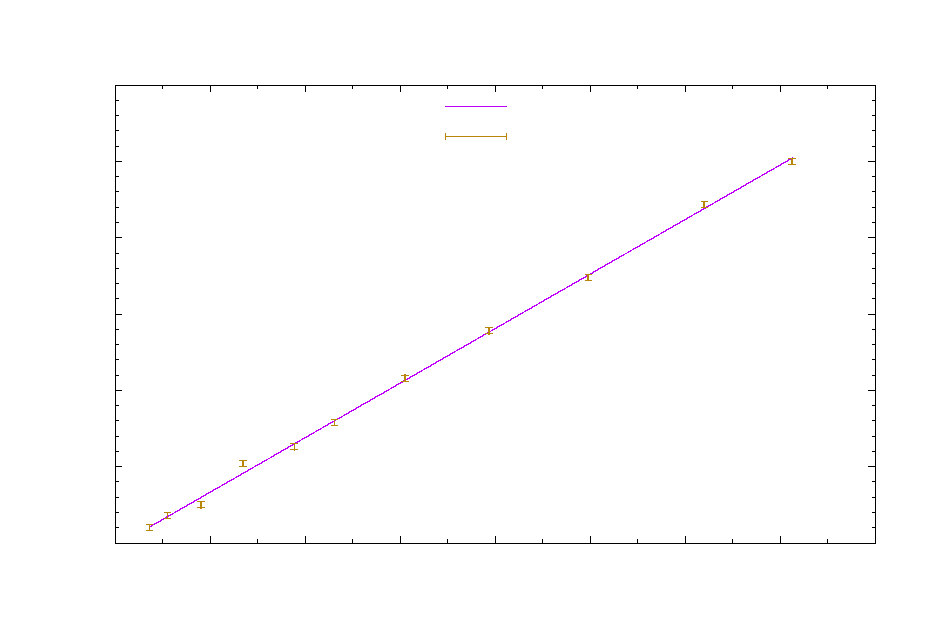
\includegraphics[width={432.00bp},height={288.00bp}]{tv5-plot}}%
    \gplfronttext
  \end{picture}%
\endgroup

		\caption{\centering Überprüfung des Stefan-Boltzmannschen Gesetzes\captionbr $\chi^2_{\text{red}} = \num{2.43832}$}
		\label{fig:tvfive-plot}
		\vspace{-1em}
	\end{figure}
	Als Endergebnis erhalten wir:
	\begin{equation*}
		\begin{tabu}{ll}
			\toprule
			b & \SI{17.8711(2133)e-10}{\micro\volt\per\kelvin^4} \\
			c & \SI{-2.420(1577)}{\micro\volt} \\
			\bottomrule
		\end{tabu}
	\end{equation*}
	Da die Auswertung mittels \gnuplot{} erfolgt, sind die Fehlerstriefen nicht gezeichnet, sondern nur als die Unsicherheit in $b$ protokolliert. 

	Aus der guten Kurveanpassung sieht man, dass das Stefan-Boltzmannsche Gesetz tatsächlich stimmt. Die Abweichungen der Punkten von der optimalen Gerade ist wahrscheinlich wegen der nicht konstante Temperatur des Räumes während des Experiments. 